\newgeometry{textwidth=16cm}
\chapter[Modélisation des interactions intermoléculaires]{Modélisation des interactions intermoléculaires}
\minitoc
\restoregeometry

\newpage

\section*{Introduction}
\markright{INTRODUCTION}{}

Les interactions non-covalentes occupent une place prépondérante dans les problématiques actuelles de recherche, celles-ci étant aujourd'hui considérées comme les pierres angulaires de disciplines telles que la chimie supramoléculaire, la science des matériaux ou la biochimie.  Au delà des liaisons hydrogènes et des interactions de nature électrostatique (\textit{e.g.} charge- charge, charge- dipôle, dipôle- dipôle), l’autre interaction non covalente la plus étudiée à l’heure actuelle est probablement celle impliquant les systèmes aromatiques \cite{grimme2008special}. Ces interactions dénommées ‘pi-stacking’ (peut être à mauvais escient (Chelsea R. Martinez and Brent L. Iverson Chem Science 2012,3, 2191-2201) entre cycles aromatiques sont notamment considérées comme responsables de la stabilité d’un très grand nombre de structures remarquables \cite{mcgaughey1998pi} dont celles qui préfigurent certainement la structures des asplhaltènes. L’étude expérimentale de ces interactions présente encore un défi car il est généralement complique de séparer les interactions $\pi$-stacking des interactions secondaires ou des effets de l’environnement. A cause de ces difficultés expérimentales, les études en chimique computationnelle apparaissent comme une alternative de choix pour comprendre la nature fondamentale des ces interactions non covalentes, ainsi que leur influence sur les systèmes chimiques étudiés. Nous encourageons le lecteur à se reporter au travail de revue Martinez et Iverson concernant ce sujet
revue dans laquelle sont recensés les principales définitions et les principaux modèles employés pour décrire ces interactions particulières.
Le graal pour les expérimentateurs comme pour les théoriciens serait d’arriver, \textit{in fine}, pouvoir caractériser séparément la contribution de chacune des ces interactions non-covalentes et d’en prévoir leur rôle et leur intensité.\\


Quoi qu’il en soit, nous savons désormais que l’énergie d'interaction intermoléculaire d'un ensemble de molécules se situe généralement entre 1 et 20 kcal/mol selon le nombre et le type de molécules impliquées. Cependant, l'énergie d'une liaison chimique covalente se mesure entre 100 et 300 kcal/mol, ce qui est d’un autre ordre de grandeur. De même, la portée d’une liaison chimique dépasse rarement quelques Angströms tandis que les interactions intermoléculaires s'étendent théoriquement jusqu'à l'infini (électrostatique) et de manière pratique entre 2 et 10 Angströms selon la taille et la nature du système.\\


D’un point de vue théorique l’énergie d’interaction intermoléculaire est une observable qu’on peut interpréter par différentes décompositions auxquelles on souhaite adjoindre, dans la mesure du possible, un sens physique. Buckingham \cite{buckingham1967permanent} proposait déjà en 1967 une décomposition de l’énergie d’interaction intermoléculaire en quatre grandes contributions : l’électrostatique $E_{elec}$, l’induction $E_{ind}$, l’echange-repulsion $E_{rep}$, et la dispersion $E_{disp}$.\\

\begin{equation}
\Delta E = E_{elec} + E_{ind} + E_{rep} + E_{disp}
\end{equation} 

L’interaction électrostatique est l’ensemble des interactions coulombiennes existant entre deux densités de charges isolées. Elle est additive et peut être répulsive ou attractive selon l’orientation relative des molécules. Elle constitue la plus grande partie de l’interaction intermoléculaire. 
 
L’énergie d’induction quand à elle due à la déformation de la densité électronique d’un atome ou d’une molécule par l’effet du champs électrique d’une molécule voisine. Cette énergie est non additive et toujours attractive.\\

Ces deux contributions sont très bien définies en physique classique, contrairement à la dispersion et à l’échange, qui sont liés à des effets quantiques.\\

La répulsion vient du principe de Pauli, qui stipule que deux électrons ne peuvent pas occuper le même spin au sein d’une même orbitale. C’est une interaction toujours répulsive et qui apparaît seulement à courte distance.\\

Finalement la dispersion n’a pas d’équivalent classique car c’est une interaction qui est liée à la corrélation électronique de deux densités de charge en interaction (fluctuation quantique des distributions de charges). Elle est attractive et existe dans tous les complexes.\\

Il y a, de façon pratique, deux manières différentes de calculer une énergie d’interaction intermoléculaire. L’une est la méthode appelée en « supermolécules », et l’autre est la méthode consistant en la construction de l’interaction intermoléculaire à partir de la connaissance des réponses des fonctions d’onde des monomères séparés (au sein du dimère) soumis à l’action de perturbations externes.\\


Dans la méthode supermoléculaire l’énergie d’interaction intermoléculaire est obtenue comme la différence entre l’énergie totale du dimère et la somme de l’énergie total de chaque monomère.


\begin{equation}
\Delta E = E_{AB} - E_{A} - E_{B} \label{eq2}
\end{equation}

A et B représentent les monomères et AB le dimère. Dans ce cas là, une erreur subtile peut se produire autour de l’énergie d’interaction. Cette erreur est connue sous le nom de Basis Set Superposition Error (BSSE) \cite{sherrill2010counterpoise}. Si nous calculons les deux monomères dans leurs bases spécifiques, et ensuite un dimère dans l’ensemble des fonctions de base des monomères, nous pourrons utiliser les orbitales virtuelles d’un monomère pour agrandir la base disponible pour la distribution de charge de l’autre monomère et vice versa. Le résultat est donc une augmentation de la qualité de la base pour le dimère vis-à-vis des monomères, et par conséquent une surestimation de l’énergie de l’interaction. Pour corriger l’erreur de BSSE, une méthode possible est de travailler dans une base complète ou saturée pour les monomères et le dimère. Une autre méthode est de calculer l’énergie des monomères dans la base du dimère, ce qui est le plus fréquemment utilisé sous le nom de counterpoise grace a Boys et Bernardi \cite{boys1970calculation}. Cette correction entraîne que pour chaque distance intermoléculaire considérée il est nécessaire de calculer l’énergie totale du dimère et des monomères.\\

L’énergie sans correction donnée pour l’équation \ref{eq2}  peut-être modifiée pour l'estimation de la quantité pour laquelle le monomère A est stabilisé artificiellement pour la base supplémentaire du monomère B et vice versa, avec la relation suivante:

\begin{equation}
E_{BASE}(A) = E_{A}^{AB}(A) - E_{A}^{A}(A)
\end{equation}

\begin{equation}
E_{BSSE}(B) = E_{B}^{AB}(B) - E_{B}^{B}(B)
\end{equation}

où l'exposant désigne la base utilisée, l'indice désigne la géométrie et le symbole entre parenthèses est le système chimique considéré.
L'énergie d'interaction corrigée est donc donnée par l'expression suivante :

\begin{equation}
E^{CP} = E_{A-B}^{A-B}(A-B) - E_{A}^{A-B}(A) - E_{B}^{A-B}(B)
\end{equation}

Dans ces conditions, les électrons de chaque fragment du système bénéficient de la base d'orbitales des autres fragments. La correction de la BSSE est par définition la différence entre l'énergie d'interaction non corrigée et l'énergie corrigée :

\begin{equation}
\Delta E^{CP} = E - E^{CP} = (E_{A-B}^{A-B}(A-B) - E_{A}^{A}(A) - E_{B}^{B}(B)) - (E_{A-B}^{A-B}(A-B) - E_{A}^{A-B}(A) - E_{B}^{A-B}(B))
\end{equation}

\begin{equation}
\Delta E^{CP} =  E_{A}^{A-B}(A) - E_{B}^{A-B}(B) - E_{A}^{A}(A) - E_{B}^{B}(B)
\end{equation}

Les bases ayant une extension spatiale finie, cette erreur est d'autant moins importante que les molécules sont éloignées les une des autres. La BSSE étant nulle dans la limite des bases infinies.
En pratique le calcul de la BSSE doit donc être effectué pour chaque conformation d’énergie minimale déterminée pour chaque distance intermoléculaire qui sépare les espèces A et B.

Plus la base est petite plus cette erreur est importante. 
Dans la limite d’une base complète la BSSE s’annule.

Les calculs HF et KS souffrent moins des effets de la BSSE (J. Garza, J.-Z. Ramírez, and R. Vargas, J. Phys. Chem. A 109, 643 (2005))
qui sont plus marqués dans les calculs post-HF (MPn, CCSD(T)), du fait en particulier du traitement de l’espace des virtuels nécessaire pour ces approches.\\


Malheureusement, le calcul direct d’une énergie d’interaction par la méthode « supermolécules » ne donne jamais aucune information sur la nature des interactions mises en jeu.\\


La première théorie qui, en mécanique quantique, a été proposé pour déterminer la nature de ces interactions intermoléculaire a été développée en dès 1927 par Wang \cite{wang1927mutual}  puis reprise et très largement étendue en 1930 par London et al \cite{london1930z}. 
Nous souhaitons, dans les paragraphes qui vont suivre rappeler en détail tous les développement de ces théories.
Nous souhaitons seulement rappeler la nature des principaux termes mis en évidence par ces auteurs. Nous avons fait le choix, dans les paragraphes qui vont suivre, de ne mener le recensement de ces termes que jusqu’aux plus bas ordres de perturbation  (les interactions de distorsion et de dispersion que l’on peut relier aux propriétés électroniques des fragments interagissant, trouvent leurs origines dans des effets du second ordre). Le choix du modèle perturbation dans notre exposé est aussi totalement arbitraire puisqu’il existe aujourd’hui de nombreux modèles autres tels ceux de  Kitaura et Morouma \cite{morokuma1977molecules} et de Stevens et Fink \cite{stevens1987frozen} pour ne citer qu’eux. Le modèle perturbatif est celui qui, à notre avis, permet la meilleur compréhension de la physique qui se cache derrière les forces de dispersion et de rendre compte des coefficients ‘dits’ de van der Waals (et des fonctions de réponses associées tels que les polarisabilités multipolaires elles même reliées aux fonctions spectrales telles que les forces d’oscillateurs et les énergies d’excitations (ref)). Enfin, le choix de présenter les termes d’interaction à partir de la théorie de perturbation nous semblait aussi justifié par le fait qu’une fois les hypothèses de travail définies et une fois les fonctions de réponses établies, la présentation des approches de type SAPT (Symetrized Adaptative Perturbation Theory) et des méthodes basées sur la détermination des fonctions semi-empiriques devant rendre compte des effets de dispersion que nous employons tout au long de ce travail s’en trouvent facilitées et justifiées.

\section[Potentiel électrostatique-Système de coordonnées]{Potentiel électrostatique - Système de coordonnées sphériques}

	Dans ce premier chapitre consacré aux interactions entre atomes à longues distances, nous allons donner les expressions générales du hamiltonien d'interaction, et établir à l'aide de la méthode de perturbation les équations du problème. Pour cela, nous utiliserons le système de coordonnées sphériques, qui, nous le verrons, est le mieux adapté à la symétrie des atomes et définirons les règles mathématiques qui en découlent.\\ 
	
	Soient deux systèmes a et b qui à l'état isolé sont susceptibles de se trouver dans les états $\phi_{0}^{a}$ ... $\phi_{p}^{a}$ et $\phi_{0}^{b}$ ... $\phi_{q}^{b}$ fonctions propres des hamiltoniens $H_{0}(a)$ et $H_{0}(b)$ correspondants aux énergies $E_{0}^{a}$ ... $E_{p}^{a}$ et $E_{0}^{b}$ ... $E_{q}^{b}$. Lorsque ces deux systèmes interagissent, le hamiltonien du système global s'écrit : 
	
	\begin{equation}
	H = H_{0}(a) + H_{0}(b) + H'
	\end{equation}
	
	Le système crée au niveau de $b$ un potentiel électrostatique $\Phi_{Kb}$ avec lequel les charges de $a$ interagissent, donnant naissance à une énergie d'interaction (et réciproquement au niveau du système $b$).
	
	\section{Ordre zéro}
	
	\subsection{Hamiltonien à l'ordre zéro pour le système [$a-b$]}
	
	A distance suffisamment grande pour que les distributions de charges liées aux systèmes a et b ne se recouvrent pas (on considère que celles-ci sont séparées), le hamiltonien à l'ordre zéro qui représente le système [$a-b$] est simplement la somme des hamiltoniens propres dus système $a$ et du système $b$. D'où : 
	
	\begin{equation}
	H_{0} = H_{0}(a) + H_{0}(b) \label{1.2}
	\end{equation}
	
	avec : 
	
	\begin{equation}
	H_{0}(a) = -\frac{1}{2} \sum_{k_{a}=1}^{n_{a}} \triangledown^{2} k_{a} - \sum_{k_{a}=1}^{n_{a}} \frac{Z_{a}}{rk_{a}} + \sum_{k'_{a}>k_{a}} \frac{1}{rk_{a},k'_{a}} + H_{l.s}(a)  \label{1.3}
	\end{equation}
	
	
	Où $\triangledown_{k_{a}}$, $Z_{a}$, $r_{k_{a}}$ et $rk_{a},k'_{a}$ représentent respectivement l'opérateur énergie cinétique, la charge du noyau de $a$, les distances noyau- électron $k_{a}$ et électron $k_{a}$- électron $k'_{a}$. L'expression de $H_{0}(b)$ se deduit facilement de celle de $H_{0}(a)$ en remplacant les coordonnées des $n_{a}$ électrons du systeme $a$ par les $n_{b}$ électrons du système $b$. $H_{l.s}(a)= \sum_{k_{a}=1}^{n_{a}} \zeta_{k_{a}} \widehat{l_{k_{a}}} \widehat{S_{k_{a}}}$ est le hamiltonien de spin-orbite de l'atome $a$, $\widehat{l_{k_{a}}}$ et $\widehat{S_{k_{a}}}$ sont les operateurs moment orbital et moment de spin de l'électron $k_{a}$, et $\zeta_{k_{a}}$ une constante de couplage spin orbite pour le même électron. 
	
	
	\subsection{Fonction d'onde moléculaire à l'ordre zéro}
	
	
	La structure électronique d'un système moléculaire et les propriétés qui en découlent peuvent être déterminées à partir de la résolution de l'équation de Schr\"{o}dinger. Pour un système constitue de $N$ électrons se déplaçant dans le champs électrostatique créé par les noyaux, cette équation s'écrit : 
	
	\begin{equation}
	H\Psi = E\Psi
	\end{equation}
	
	La résolution de l'équation intégro-différentielle de Schr\"{o}dinger aux états stationnaires pour les systèmes pluriélectroniques n'est pas envisageable sans approximations. Les fonctions propres du hamiltonien $H$ décrivent les états du systèmes dont l'énergie est égale à la valeur propre correspondante. De l'expression \ref{1.2} du hamiltonien non perturbé, une expression de la fonction d'onde $\Psi_{00}$ décrivant l'interaction entre deux atomes $a$ et $b$ pris dans leur état fondamental peut être : 
	
	\begin{equation}
	\Psi_{00} = \phi_{0}^{a} \cdot \phi_{0}^{b}
	\end{equation}
	
	Produit non antisymétrisé des fonctions d'ondes $\phi_{0}^{a}$ et $\phi_{0}^{b}$ des systèmes $a$ et $b$ non perturbés. En toute rigueur, le simple produit des fonctions $\phi_{0}^{a}$ et $\phi_{0}^{b}$ n'est pas correct au vu des lois de la mécanique quantique puisque le principe d'indicernabilité n'est pas vérifié. Néanmoins, pour les grandes distances interatomiques pour lesquelles les électrons ne peuvent s'échanger d'un atome à l'autre, on pourra dans ce cas, négliger le recouvrement entre les fonctions d'onde atomiques (et par conséquence de ne pas tenir compte des termes d'échanges).\\
	
	Le dernier terme de l'expression \ref{1.3} $H_{l.s}(a) = \sum_{k_{a}=1}^{n_{a}} \zeta_{k_{a}} \widehat{l_{k_{a}}} \widehat{S_{k_{a}}}$ représente le couplage spin orbite qui rend compte de l'interaction entre les deux dipôles magnétiques produite respectivement par le spin et le mouvement de chacun des électrons sur son orbite. Ce terme est de nature relativiste. Dans ce travail, nous négligerons les interactions des spins avec les orbites des autres spins, ainsi que les interactions spin- spin, approximation qui est d'autant plus justifiée que le terme répulsif est faible. Nous nous placerons donc toujours dans le cas d'un couplage (a) de Hund \cite{bussery1989semi}. Cette approximation est appelée "non couplée" \cite{fontana1961theory,fontana1962theory} et les fonctions d'onde moléculaires correspondante qui représentent le système [$a-b$] auront pour expression générale : 
	
	\begin{equation}
	\Psi_{00}^{\nu} = \sum_{k=1}^{n_{\nu}} \alpha_{\nu k}| S_{k} L_{k} M_{S_{k}} M_{L_{k}} \rangle _{a} | S'_{k} L'_{k} M'_{S_{k}} M'_{L_{k}} \rangle _{b}
	\end{equation}
	
	Où $S_{k}$, $L_{k}$, $M_{S_{k}}$ et $M_{L_{k}}$ representent les nombres quantiques de spin, orbitalaire et magnetiques de l'atome $a$. L'indice prime sera réservé au système $b$. 
	
	
	\subsection{Perturbation}
	
	Deux atomes ou molécules à couches fermées manifestent toujours une énergie d'interaction due aux forces de Van der Waals. Cette énergie d'interaction sera calculée, dans ce travail, à l'aide d'une méthode de perturbation puisqu'elles représente aux grandes distances interatomiques $R$, la différence très faible entre deux énergies voisines $E_{ab}(R)$ (avec $R$ grand devant $R_{eq}$) et $E_{ab}(\infty)$ qui est l'énergie des deux entités séparées d'une distance à laquelle aucune interaction n'existe.\\
	
	Tout le problème consiste donc à évaluer le déplacement de l'état fondamental du à l'introduction de $H'$ et particulier sa dépendance en $R$. L'interaction coulombienne $V$, entre les électrons et le noyau de $a$ et les électrons et le noyau de $b$ sera traitée comme une perturbation en considerant que $H'$ reste faible devant le hamiltonien du système global isolé ($H_{0}(a)+ H_{0}(b)$). 
	
	\begin{equation}
	V = - \sum_{k_{a}=1}^{n_{a}} \frac{Z_{b}}{r_{bk_{a}}} - \sum_{k_{b}=1}^{n_{b}} \frac{Z_{a}}{r_{ak_{b}}} + \sum_{k_{a}=1}^{n_{a}} \sum_{k_{b}=1}^{n_{b}} \frac{1}{r_{k_{a}k_{b}}} + \frac{Z_{a} Z_{b}}{R}
	\end{equation}
	
	
	\section{Le Hamiltonien d'interaction}
	
	
	Soit un système dans lequel les charges sont localisées. Le hamiltonien d'interaction $H'$ s'exprime en fonction du potentiel électrostatique [$\Phi_{K_{b}}= \sum_{k_{a}=1}^{N_{a}} \frac{e_{k_{a}}}{r_{k_{a}}}$] subi par les charges du système $b$ vis à vis des charges du système $a$ (ou réciproquement par son équivalent $\Phi_{K_{a}}$ relatif au système $a$).
	
	\begin{equation}
	H' = \sum_{k_{b}=1}^{N_{b}} e_{k_{b}} \Phi_{k_{b}} = \sum_{k_{a}=1}^{N_{a}} \sum_{k_{b}=1}^{N_{b}} \frac{e_{k_{a}} e_{k_{b}}}{r_{k_{a}k_{b}}}
	\end{equation}
	
	En développant le potentiel $\Phi_{K_{b}}$ en série de Taylor par rapport au centre de la distribution de charges de $b$ (noté "o") :
	
	\begin{equation}
	\Phi_{K_{b}} = \Phi_{o} + (\triangledown_{\alpha} \Phi)_{o} r_{K_{b}\alpha} + \frac{1}{2} (\triangledown_{\alpha} \triangledown_{\beta} \Phi)_{o} r_{K_{b}\alpha} r_{K_{b}\beta} + \ldots
	\end{equation}
	
	On obtient pour expression de $H'$ : 
	
	\begin{equation}
	H' = \sum_{K_{b}=1}^{N_{b}} e_{K_{b}} \left(\Phi_{o} + (\triangledown_{\alpha} \phi)_{o} r_{K_{b}\alpha} + \frac{1}{2}(\triangledown_{\alpha} \triangledown_{\beta}\phi)_{o} r_{K_{b}\alpha} r_{K_{b}\beta} + \ldots \right)
	\end{equation}
	
	Où $\alpha,\beta=$ (x, y ou z) et où l'indice $k_{b}$ se rapporte indifféremment au noyau et aux électrons du système $b$ ($N_{b}$). $\triangledown_{\alpha}$ correspond à une des trois composantes de l'opérateur gradient ($\frac{\partial}{\partial x}, \frac{\partial}{\partial y} ou \frac{\partial}{\partial z}$) et $r_{K_{b}\alpha}$ à la composante du rayon vecteur représentant la particule $k_{b}$. En tenant compte des définitions des moments multipolaires centrés sur l'origine du système : 
	
	\begin{flushleft}
		\begin{equation*}
		\sum_{k_{b}=1}^{N_{b}} e_{k_{b}} = q^{b} \hspace{8.1cm}\textup{charge électrique de la molecule $b$}     
		\end{equation*}
	\end{flushleft}
	
	\begin{flushleft}
		\begin{equation*}
		\sum_{k_{b}=1}^{N_{b}} e_{k_{b}} r_{k_{b}\alpha} = \mu_{\alpha}^{b}  \hspace{4.8cm} \textup{composante du moment dipolaire de $b$ à l'origine}
		\end{equation*}
	\end{flushleft}
	
	
	\begin{flushleft}
		\begin{equation*}
		\frac{1}{2} \sum_{k_{b}=1}^{N_{b}} e_{k_{b}} (3r_{k_{b}\alpha} r_{k_{b}\beta}- r^{2}_{k_{b}}\delta_{\alpha \beta}) = \theta_{\alpha \beta}^{b}  \hspace{1cm} \textup{élément $\alpha\beta$ du tenseur moment quadripolaire de $b$}
		\end{equation*}
	\end{flushleft}
	
	Ainsi que des définitions du champ :
	
	\begin{equation}
	F_{\alpha}^{b} = - \left(\frac{\partial \phi_{k_{b}}}{\partial r_{\alpha}}\right)_{o} = - (\triangledown_{\alpha} \phi_{k_{b}})_{o} \label{1.11}
	\end{equation}
	
	et du gradient du champ électrique en "o" : 
	
	\begin{equation}
	F_{\alpha\beta}^{b} = - \left(\frac{\partial^{2} \phi_{k_{b}}}{\partial r_{\alpha} \partial r_{\beta}}\right)_{o} = - (\triangledown_{\alpha} \triangledown_{\beta} \phi_{k_{b}})_{o} \label{1.12}
	\end{equation}
	
	on retrouve l'expression classique du hamiltonien d'interaction : 
	
	\begin{equation}
	H' = \Phi_{o} q^{b} - \sum_{\alpha} F_{\alpha}^{b} \mu_{\alpha}^{b} - \frac{1}{3} \sum_{\alpha\beta} F_{\alpha\beta}^{b} \theta_{\alpha\beta}^{b} + \ldots
	\end{equation}
	
	En posant le vecteur $\overrightarrow{R_{k}}= \overrightarrow{R} - \overrightarrow{r_{k}}$ qui représente la distance de la particule $k$ à l'origine de la distribution de charges, le potentiel $\Phi_{o}$ créé en "o" peut s'écrire soit sous sa forme classique \ref{1.14}:
	
	\begin{equation}
	\Phi_{o} = \frac{q^{a}}{R} + \sum_{\alpha} \mu_{\alpha}^{a} \frac{R_{\alpha}}{R^{3}} + \sum_{\alpha\beta} \theta_{\alpha,\beta}^{a} \frac{R_{\alpha} R_{\beta}}{R^{4}} + \ldots \label{1.14}
	\end{equation}
	
	soit sous une forme plus simplifiée : 
	
	\begin{equation}
	\Phi_{o} = q^{a} T - \sum_{\alpha} \mu_{\alpha}^{a} T_{\alpha} + \sum_{\alpha\beta} \theta_{\alpha\beta}^{a} T_{\alpha\beta} + \ldots
	\end{equation}
	
	
	dans laquelle, les quantités $T$, $T_{\alpha}$ et $T_{\alpha\beta}$ sont posées égales à :
	
	\begin{equation}
	\begin{cases}
	T = R^{-1} \\
	T_{\alpha} = \triangledown_{\alpha} R^{-1} = - \frac{R_{\alpha}}{R^{3}}\\
	T_{\alpha\beta} = \triangledown_{\alpha} \triangledown_{\beta} R^{-1} = \frac{3R_{\alpha} R_{\beta}- R^{2}\delta_{\alpha\beta}}{R^{5}}
	\end{cases}
	\end{equation}
	
	$F_{\alpha}^{b}$ \ref{1.11} et $F_{\alpha\beta}^{b}$ \ref{1.12} sont exprimées en fonction des moments multipolaires [$4-6$] précédemment définis : 
	
	\begin{equation}
	F_{\alpha}^{b} = -(\triangledown_{\alpha}\phi_{B})_{o} = -q^{a} T_{\alpha} + \mu_{\alpha}^{a} T_{\alpha\beta} - \frac{1}{3} \theta_{\beta\gamma}^{a} T_{\alpha\beta\lambda} + \ldots 
	\end{equation}
	
	\begin{equation}
	F_{\alpha\beta}^{b} = -(\triangledown_{\alpha} \triangledown_{\beta}\phi_{B})_{o} = q^{a} T_{\alpha\beta} + \mu_{\delta}^{a} T_{\alpha\beta\lambda} - \frac{1}{3} \theta_{\gamma\delta}^{a} T_{\alpha\beta\gamma\delta} + \ldots 
	\end{equation}
	
	Le hamiltonien d'interaction devient alors : 
	
	\begin{equation}
	H' = q^{a} q^{b} T + T_{\alpha}(q^{a} \mu_{\alpha}^{a}) + T_{\alpha\beta} (\frac{1}{3}q^{a}\delta^{b}_{\alpha\beta}+ \frac{1}{3} q^{b}\delta^{a}_{\alpha\beta} - \mu_{\alpha}^{a}\mu_{\beta}^{b}) + \ldots  \label{1.19}
	\end{equation}
	
	$H'$ apparait comme la somme d'une infinité de termes : 
	
	\begin{itemize}
		\item contribution de la charge totale du système : $\frac{q^{a}q^{b}}{R}$. Ce terme représente le potentiel en ($1/R$) que créent les charges des systèmes $a$ et $b$.
		
		\item contribution du moment dipolaire électrique du système : interaction charge de $a$ - moment dipolaire de $b$ et charge de $b$ - moment dipolaire de $a$. Au total, on obtient un terme variant en $T_{\alpha}$ soit en ($1/R^{2}$).
		
		\item un terme d'interaction dipôle dipôle et deux termes charge de $a$ - quadrupole de $b$ et charge de $b$ -quadrupole de $a$ variant en ($1/R^{3}) \ldots$
	\end{itemize}
	
	La première contribution au potentiel d'interaction des moments multipolaires sera généralement due au terme d'interaction dipôle- dipôle variant en ($1/R^{3}$). Aux grandes distances interatomiques, la contribution des termes au développement \ref{1.19} décroit très vite et seuls les premiers termes suffisent à exprimer le potentiel d'interaction. Nous verrons dans les applications les conséquences que cela entraine sur le développement de l'énergie d'interaction, dont l'expression analytique sera obtenue à l'aide des termes de Van der Waals ($C_{3}, C_{5}, C_{6}, \ldots$).
	
	\section{La théorie de perturbations}
	
	Le système de coordonnées cartésiennes est le système le plus utilisé et le plus naturel puisqu'il s'appuie sur la tri-dimensionnalité de notre espace quotidien. Néanmoins, son utilisation devient très vite complexe lorsque l'on veut traiter des propriétés d'interaction. Il existe un autre système de référence plus adapte à l'étude de ce type de propriétés qui s'appuie sur le principe simple de proportionnalité entre les harmoniques sphériques. Ce référentiel est le système de coordonnées sphériques. Nous étudierons dans ce chapitre, le développement à un et deux centres du potentiel électrostatique dû à une distribution de charges discrètes, puis nous montrerons quelles sont les transformations nécessaires pour passer d'un système de coordonnées à l'autre. 
	
	\subsection{Développement à un centre du potentiel électrostatique dû à une distribution de charges discrètes}  
	
	Soit $\Phi_{\rho}$, le potentiel électrostatique créé par une distribution de charges centrée en A, pour un point $\rho$ qui lui est extérieur : 
	
	\begin{equation}
	\Phi_{\rho} = \sum_{k_{a}=1}^{n_{a}} \frac{e_{k_{a}}}{r_{k_{a}\rho}} \label{1.20}
	\end{equation}
	
	$e_{k_{a}}$ représente la charge de la $k_{a}^{eme}$ particule et $r_{k_{a}\rho}$ la distance qui sépare cette charge du point $\rho$ considéré. Le développement de $\Phi_{\rho}$ sera effectué dans le système de coordonnées sphériques. Pour cela, nous utiliserons la formulation de Laplace pour développer la quantité $\frac{1}{r_{k_{a}\rho}}$.
	
	\begin{equation}
	\frac{1}{r_{k_{a}\rho}} = \sum_{i=0}^{\infty} \sum_{m=-i}^{+i} \frac{(i-|m|)!}{(i+ |m|)!} \frac{r^{i}<}{r^{i+1}>} P_{m}^{i} (\cos\theta_{k_{a}}) P^{i}_{m}(\cos\theta_{\rho})e^{im(\phi_{k_{a}}- \phi_{\rho})} \label{1.21}
	\end{equation}
	
	où $r< =$ min. $\{r_{k_{a}}, r_{\rho}\} \equiv r_{k_{a}}$
	$r> =$ max. $\{r_{k_{a}}, r_{\rho}\} \equiv r$
	
	et où les termes $P_{m^{i}} (\cos\theta_{\rho})$ représentent les fonctions associées au polynôme de Legendre de première espèce. Ces fonctions s'identifient aux harmoniques sphériques $Y_{i}^{m}(\theta,\phi)$ à un facteur près : 
	
	\begin{equation}
	P_{m}^{i}(\cos\theta) = (-1)^{m-|m|} \frac{\sqrt{4\pi}}{\sqrt{2i+ 1}} \frac{\sqrt{(i+ |m|)!}}{\sqrt{(i-|m|)!}} e^{-im\phi} Y_{i}^{m}(\theta,\phi) \label{1.22}
	\end{equation}
	
	D'après les équations \ref{1.21} et \ref{1.22}, le développement de la Laplace pour l'inverse de la distance $r_{k_{a}\rho}$ entre la charge $q_{a}$ appartenant à la distribution $a$ et le point $\rho(r_{\rho}, \theta_{\rho}, \phi_{\rho})$ qui lui est extérieur, s'exprime comme : 
	
	\begin{equation}
	\frac{1}{r_{k_{a}\rho}} = \sum_{i=0}^{\infty} \sum_{m=-i}^{+i} (-1)^{|m|} \frac{4\pi}{2i +1} \frac{r_{k_{a}}^{i}}{r_{\rho}^{i+1}} Y^{m}_{i} (\theta_{k_{a}}, \phi_{k_{a}}) Y_{i}^{-m} (\theta_{\rho},\phi_{\rho})  \label{1.23}
	\end{equation}
	
	
	En remplaçant l'expression \ref{1.23} dans la formulation du potentiel électrostatique \ref{1.20}, l'expression de $\Phi_{\rho}$ dépend de $\theta$ et $\phi$ : 
	
	\begin{equation}
	\Phi_{\rho} = \sum_{i=0}^{\infty} \sum_{m=-i}^{+i} (-1)^{|m|}\frac{4\pi}{2i +1} \frac{1}{r_{\rho}^{i+1}} Y_{i}^{-m} (\theta_{\rho},\phi_{\rho}) \sum_{k_{a}} e_{k_{a}}r^{i}_{k_{a}} Y^{m}_{i} (\theta_{k_{a}}, \phi_{k_{a}})
	\end{equation}
	
	dans laquelle, pour simplifier l'écriture, nous poserons la variable $Q_{m}^{i}(a)$ égale à : 
	
	\begin{equation}
	Q_{m}^{i}(a)= \frac{\sqrt{4\pi}}{\sqrt{2i + 1}} \sum_{k_{a}} e_{k_{a}}r_{k_{a}}^{i} Y_{i}^{m} (\theta_{k_{a}}, \phi_{k_{a}}) \label{1.25}
	\end{equation}
	
	\begin{equation}
	\Phi_{\rho} = \sum_{i=0}^{\infty} \sum_{m=-i}^{+i} (-1)^{|m|} \frac{4\pi}{2i +1} \frac{1}{r_{\rho}^{i+1}} Y_{i}^{-m} (\theta_{\rho},\phi_{\rho})Q_{m}^{i}(a)
	\end{equation}
	
	Physiquement, les quantités $Q_{m}^{i}(a)$ représentent les combinaisons linéaires des composantes des opérateurs moments polaires du système $a$. 
	
	
	\begin{itemize}
		\item i=0 m=0 \hspace{0.9cm} $Q_{0}^{0}(a) = \sum_{k_{a}} e_{k_{a}} = q^{a}$ \hspace{3.5cm} charge de $a$
		
		\item i=1 m=0 \hspace{0.9cm} $Q_{_{0}^{1}}(a)= \sum_{k_{a}} e_{k_{a}} r_{k_{a}} P^{0}_{1} (\cos\theta_{k_{a}}) = \mu_{z}^{a}$ \hspace{1cm} composante z de l'opérateur
		
		\item i=1 m=1 \hspace{0.9cm} $Q_{1}^{1}(a)= \sum_{k_{a}} \frac{1}{\sqrt{2}}e_{k_{a}} r_{k_{a}} P^{1}_{1} (\cos\theta_{k_{a}}) e^{i\phi k_{a}}$ \hspace{0.6cm} moment dipolaire de l'atome $a$
		
		\item i=1 m=-1 \hspace{0.9cm} $Q_{-1}^{1}(a) = -\sum_{k_{a}} \frac{1}{\sqrt{2}}e_{k_{a}} r_{k_{a}} P^{1}_{-1} (\cos\theta_{k_{a}}) e^{-i\phi k_{a}}$
	\end{itemize}
	
	Si l'on considère que l'axe $z$ est l'axe de plus haute symétrie, les formulations des composantes perpendiculaires $x$ et $y$ du moment dipolaire électrique du système sont : 
	
	\begin{equation}
	\mu_{x}^{a} = \frac{1}{\sqrt{2}} (Q_{1}^{1}(a)- Q_{-1}^{1}(a)
	\end{equation}
	
	\begin{equation}
	\mu_{y}^{a} = \frac{1}{\sqrt{2i}} (Q_{1}^{1}(a)+ Q_{-1}^{1}(a)
	\end{equation}
	Les autres composantes du tenseur d'ordre deux seront obtenues en remplaçant $m$ par ses valeurs permises ($m=\pm 1, m=\pm 2$).
	
	Les propriétés de ces opérateurs sont indépendantes du système étudié et satisfont à un ensemble de règles de sélections sur lesquelles nous reviendrons. 
	
	\begin{itemize}
		\item l=2 m=0 \hspace{1cm} $Q_{0}^{2}(a) = \theta_{zz}^{a}$ \hspace{1cm} composante $z$ de l'opérateur moment quadripolaire 
	\end{itemize}
	
	
	\subsection{Développement à deux centres de l'interaction coulombienne entre deux distributions de charges ne se recouvrant pas}
	
	De nombreux travaux \cite{buehler1951bipolar,hylleraas1931elektronenterme,proctor1977long,davison1968atomic} ont montré que l'inverse de la distance $r_{ij}$, distance de la charge $i$ à la charge $j$, peut s'écrire sous forme d'un développement bipolaire dans le système de coordonnées de deux distributions (système de coordonnées bipolaires).
	
	\begin{equation}
	\frac{1}{r_{k_{a}k_{b}}} = \sum_{i,j=0}^{\infty} \sum_{-l<}^{l>} B_{ij}^{|m|}(r_{k_{a}}, r_{k_{b}}; R) P_{i}^{m} (\cos\theta_{k_{b}}) P_{j}^{m}(\cos\theta_{k_{a}}) e^{im(\phi_{k_{a}}-\phi_{k_{b}})}
	\end{equation}
	
	$l< = inf.(i,j)$
	
	
	Dans l'hypothèse où les deux distributions de charges ne se recouvrent pas, on peut considérer que $R> r_{i} +r_{j}$ et poser : 
	
	\begin{equation}
	B_{ij}^{|m|}(r_{k_{a}}, r_{k_{b}}; R) = \frac{(1-)^{j+|m|} (i+j)!}{(i+|m|)! (j+|m|)!} r^{i}_{k_{a}} r_{k_{a}}^{j} \frac{1}{R^{i+j+1}}
	\end{equation}
	
	Le potentiel d'interaction entre les deux distributions de charges s'écrit : 
	
	\begin{equation}
	V = \sum_{k_{a}=1}^{N_{a}} \sum_{k_{b}=1}^{N_{b}} \frac{e_{k_{a}}e_{k_{b}}}{r_{k_{a}k_{b}}}
	\end{equation}
	
	
	Le polynôme associe de Legendre s'exprime en fonction des harmoniques sphériques : 
	
	\begin{equation}
	V = \sum_{i,j=0}^{\infty} \frac{1}{R^{i+j+1}} \sum_{-l<}^{l>} \frac{(-1)^{j} (i+j)!} {\sqrt{(i+m)! (i-m)! (j-m)! (j+m)!}}
	\end{equation}
	
	\begin{equation}
	\frac{\sqrt{4\pi}}{\sqrt{2i}+ 1} \sum_{k_{a}=1}^{N_{a}} e_{k_{a}} r_{k_{a}}^{i} Y_{i}^{m} (\theta_{k_{a}},\phi_{k_{a}}) \frac{\sqrt{4\pi}}{\sqrt{2j+ 1}} \sum_{k_{b}=1}^{N_{b}} e_{k_{b}}r_{k_{b}}^{j} Y_{j}^{-m}(\theta_{k_{b}},\phi_{k_{b}})
	\end{equation}
	
	Où $V$ se développe en fonction des opérateurs moments multipolaires de $a$ et de $b$ définis par la relation \ref{1.25}.
	
	En posant la quantité $\frac{(-1)^{j} (i+j)!} {\sqrt{(i+m)! (i-m)! (j-m)! (j+m)!}}$ égale à $d_{m}(i,j)$ on obtient pour expression simplifiée du potentiel d'interaction l'équation générale suivante : 
	
	\begin{equation}
	V = \sum_{i,j=0}^{\infty} \frac{1}{R^{i+j+1}} \sum_{-l<}^{l>} d_{m}(i,j) Q_{m}^{i}(a) Q_{-m}^{j} (b) = \sum_{i=0}^{\infty} \sum_{j=0}^{\infty} \frac{V_{ij}(a,b)}{R^{i+j+1}} \label{1.33}
	\end{equation}
	
	Les opérateurs multipolaires $Q_{m}^{i;j}$ (charge, dipôle, quadripôle,...) contiennent toute l'information sur la distribution de charges du système considéré. Le potentiel $V(a,b)$ contient donc chacune des ces informations pour chacun des deux systèmes $a$ et $b$ pris isolément. En prenant l'ensemble des valeurs de $i$ et $j$ permises, les différentes interactions intervenant entre les multipôles des deux systèmes (induit ou permanent) sont :
	
	\begin{itemize}
		\item i = j = 0 $V_{00}$ représente l'interaction entre la charge de $a$ et la charge de $b$. Ce terme est nul pour les systèmes neutres. 
		
		\item i = 0 et j = 1 $V_{01}$ représente l'interaction entre la charge de $a$ et le dipôle de $b$. 
		
		\item i = j = 1  $V_{11}$ représente l'interaction entre le dipôle de $a$ et le dipôle de $b$.
	\end{itemize}
	
	i et j prennent des valeurs théoriquement infinies, mais nous verrons que l'expression \ref{1.33} peut être tronquée pour des valeurs de i et j faibles. De plus, suivant la nature des espèces en présence, toutes les combinaisons des paramètres i et j ne sont pas permises. Ces règles de sélection sont fournies par les règles sur les symboles "3j".
	
	
	\chapter*{Energie d'interaction}
	
	Cette partie est consacré au recensement de l'ensemble des termes d'interaction obtenus à partir d'un calcul au premier et au second ordre de perturbation ainsi qu'à celui des termes prépondérants d'ordre 6 et 8 que nous pouvons estimer \cite{saute1982calculated}.
	
	\section{Calcul de l'energie électrostatique}	
	
	\subsection{Expression des éléments de matrice de l'énergie électrostatique}
	
	L'énergie électrostatique représente l'énergie calculée au premier ordre des perturbation 
	
	\begin{equation}
	E_{1} = \langle \psi_{00}^{\nu}|V| \psi_{00}^{\lambda}\rangle
	\end{equation}
	
	
	En remplaçant l'opérateur $V_{ij}$ de perturbation par son expression \ref{1.33}, l'énergie électrostatique d'un système [$a-b$] s'exprime sous la forme d'une suite infinie : 
	
	\begin{equation}
	E = \sum_{i=0}^{\infty} \sum_{j=0}^{\infty} \frac{E_{ij} (\nu,\lambda)}{R^{i+j+1}} = \sum_{m} \frac{C_{m}}{R^{m}}
	\end{equation}
	
	dans laquelle les coefficients $C_{m}$ representent directement les éléments de matrices $E_{ij}$ de l'énergie d'interaction électrostatique entre deux états $\nu$ et $\lambda$ : 
	
	\begin{equation}
	E_{ij}(\nu, \lambda) = \langle \psi_{00}^{\nu}|V_{ij}(a,b)|\psi_{00}^{\lambda} \rangle = C_{m}
	\end{equation}
	
	où $m= i+j+1$ 
	
	En reprenant les expressions des fonctions d'ondes :
	
	\begin{equation}
	F_{l}^{m} (\theta,\phi) = \lambda (l)Y_{l}^{m} (\theta,\phi)
	\end{equation}
	
	Les éléments de matrices $E_{ij}$ s'expriment en fonction du terme d'interaction induit par les multipôles électrostatiques de $a$ et de $b$ : 
	
	\begin{equation*}
	E_{ij} (\nu , \lambda) = \sum_{k=1}^{n_{\nu}} \sum_{l=1}^{n_{\lambda}} \alpha_{\nu k} \alpha_{\lambda l}
	\end{equation*}
	
	\begin{equation}
	\langle S_{k}L_{k}M_{S_{k}}M_{L_{k}}|\langle S'_{k}L'_{k}M'_{S_{k}}M'_{L_{k}}| V_{ij}(a,b)| S_{l}L_{l}M_{S_{l}} M_{L_{l}} \rangle S'_{l}L'_{l}M'_{S_{l}}M'_{L_{l}} \rangle
	\end{equation}
	
	avec 
	
	\begin{equation}
	V_{ij}(a,b) = \sum_{m=-l<}^{l>} d_{m}(i,j) Q_{m}^{i}(a) Q_{-m}^{j}(b) 
	\end{equation}
	
	
	Ce terme $V_{ij}$ apparaît comme le produit d'un opérateur tensoriel irréductible de rang $i$ n'agissant que sur les seules coordonnées de $a$, par un autre opérateur tensoriel irréductible, de rang $j$, n'agissant que sur les coordonnées de $b$. Dans le cadre de cette propriété, les éléments de matrices de l'énergie électrostatique se décomposent en deux parties : l'une relative au système $a$ et l'autre relative au système $b$. 
	
	\begin{equation*}
	E_{ij}(\nu , \lambda)= \sum_{k=1}^{n_{\nu}} \sum_{l=1}^{n_{\lambda}} \alpha_{\nu k} \alpha_{\lambda l} \sum_{m=-l<}^{l>} d_{m}(i,j)
	\end{equation*}
	
	
	\begin{equation}
	\langle S_{k}L_{k}M_{S_{k}}M_{L_{k}}| Q_{m}^{i} (a)| S_{l}L_{l}M_{S_{l}}M_{L_{l}}\rangle \langle S'_{k}L'_{k}M'_{S_{k}}M'_{L_{k}}| Q_{-m}^{j} (b) | S'_{l}L'_{l}M'_{S_{l}}M'_{L_{l}}\rangle
	\end{equation}
	
	Il est possible de simplifier notablement cette expression en utilisant les propriétés du théorème de Wigner- Eckart (WE).
	
	
	\subsection{Application des règles de sélection à la détermination des coefficients de dispersion $C_{m}$}
	
	Les règles de sélection nous ont conduis aux relations :
	
	\begin{equation}
	\begin{cases}
	L_{k} + i + L_{l} = entier\ pair \\
	|L_{k} - L_{l}| \leq i \leq L_{k} + L_{l} \\
	L'_{k} + j + L'_{l} = entier\ pair \\
	|L'_{k} - L'_{l}| \leq j \leq L'_{k} + L'_{l}
	\end{cases}
	\end{equation}
	
	
	\begin{itemize}
		\item Si $L_{k} + L_{l}$ est paire, $i$ est nécessairement paire (idem pour $j$). $i + j$ est donc paire.
		
		\item Si $L_{k} + L_{l}$ est impaire $i$ est nécessairement impaire (idem pour j). $i + j$ est encore paire.
	\end{itemize}
	
	
	Ainsi, on peut dire que quelles sue soient les valeurs des moments orbitaux, $i + j$ est toujours paire. L'énergie électrostatique : 
	
	\begin{equation}
	E(l) = \sum_{n=0}^{\infty} \frac{C_{i+j+1}}{R^{i+j+1}}
	\end{equation}
	
	sera donc toujours représentée par un développement en puissance impaire $i+ j + 1$ de $R$.
	
	\begin{itemize}
		\item Si deux atomes identiques ou non, de même spin ou non, sont tous les deux dans un état initial de symétrie $S$ : $L_{k} = L_{l} = L'_{k} = L'_{l} = 0$, nous aurons donc : 
		
		\begin{equation*}
		\begin{cases}
		0 + i + 0 = entier\ pair \\
		|0 - 0| \leq i \leq 0 + 0 \\
		0 + j + 0 = entier\ pair \\
		|0 - 0| \leq j \leq 0 + 0
		\end{cases}
		\end{equation*}
		soit $i = j = 0$; interaction charge-charge ($Q_{0}^{0}- Q_{0}^{0}$). 
		
		\item Si deux atomes identiques ou non, de même spin ou non, tel qu'un des deux se trouve dans un état de symétrie $S$ et l'autre dans un état de symétrie $P$ sont en interaction : $L_{k} = L_{l} = 0$, $L'_{k} = L'_{l} = 1$, alors les sommes $i + 1$ et $j + 1$ sont entières et paires. Soit $i = j = 1$. L'énergie électrostatique possède donc un terme de résonance non nul d'ordre trois : $C_{3}/R^{3}$. 
		
		\item Si deux atomes identiques ou non, de même spin ou non, se trouvent dans un état de symétrie $P$ et sont en interaction : $L_{k} = L_{l} = L'_{k} = L'_{l} = 1$, alors $i + 2$ et $j + 2$ sont entières et paires. Ces règles impliquent que $i = j = 2$. L'énergie électrostatique possède un terme d'ordre cinq non nul : $C_{5}/R^{5}$. 
		
	\end{itemize}
	
	
	
	
	
	\begin{itemize}
		\item Dans le cas d'interaction de type $S + S : l_{k} = l_{l} = 0$ et $ L'_{k} = L'_{l} = 0$ on a $i = i' = l"_{a}$ et $j= j' = 0$. Les combinaisons (i,i',j,j') permises seront celles pour lesquelles $i = i'$; (i,i,0,0). La somme $i = i'$ est paire. Les termes d'induction sont donc paires d'ordre 4. Ces termes représentent les interactions dipôle d $a$ - charge de $b$, quadrupôle de $a$ - charge de $b$, etc... et sont toujours nuls dans le cas des atomes neutres. Il est bien évident que le résultat serait le même si nous avions pris les états excités de $b$ plutôt que ceux de $a$. 
		
		\item Dans le cas d'interaction de type $S + P$, plusieurs cas de figures sont à envisager :
		
		On fait l'hypothèse de toujours raisonner sur les états excités de $a$ et sur l'état initial de $b$. La réciproque doit être envisagée pour traiter de la contribution de l'énergie d'induction dans son ensemble. 
		
		Dans le cas où l'atome $a$ est de symétrie $P (l_{k} = l_{l} = 1)$ et l'atome $b$ de symétrie $S (l'_{k} = l'_{l} = 0)$ les règles de sélection amènent pour $b$ aux mêmes conclusions que dans le cas précédent (j = j' = 0). Ce terme est toujours nul dans le cas des atomes neutres. 
		
		Dans le cas où l'atome $a$ est de symétrie $S (l_{k} = l_{l} = 0)$ et l'atome $b$ de symétrie $P (l'_{k} = l'_{l} = 1)$ les règles de sélections nous donnent pour $b$ (j=0, 2 et j'=0, 2) et pour $a$ (i = i'). Dans ce cas, les combinaisons permises sont (1,1,2,2) pour le terme d'ordre 8, (2,2,2,2) pour le terme d'ordre 10, etc. [la valeur 0 est interdite pour les atomes neutres]. Le premier terme qui contribue à la valeur de l'énergie d'induction est donc le terme d'ordre 8 ($C_{8}$) et l'expression de cette dernière prend la forme : 
		
		\begin{equation}
		E_{ind}^{ii'22} (a;\nu , \lambda) = \sum_{i=i'=1}^{\infty} \frac{C_{i+i'+6}}{R^{i+i'+6}} \hspace{2cm} avec \hspace{0.5cm} j = 2
		\end{equation}
		
	\end{itemize}
	
	
	
   \section{SAPT}
   \markright{SAPT}{}
   
   Comme nous l’avons déjà mentionné les interactions de van der Waals ne sont clairement distinctes des
   autres types d’interactions qu’à longues distances. Dans la région intermédiaire, qui inclut la région du
   minimum, il est même particulièrement difficile de décomposer de manière univoque l’énergie totale d’interaction
   en différentes contributions. Plusieurs schéma de décomposition ont néanmoins été proposés au fil du temps.
   Parmi ces schémas citons les approches du type ‘supermolécule’ ou encore les approches basées sur la théorie des perturbations de Rayleigh-Schr\"{o}dinger comme celle que nous avons développée au chapitre —. 
   Le principe de ces dernières approches est d’évaluer par morceaux les différentes contributions, telles que l’électrostatique, l’induction, la dispersion.
   Leur défaut majeur est qu’elles conduisent à des processus non convergés (ou mal convergés) de la série perturbationnelle du fait à la fois de leur troncature à des ordres souvent pris comme trop bas 
   et du fait de leur non complétude.
   C’est pour palier à ce dernier défaut que la théorie SAPT (Symmetry Adapted Perturbation Theory) a été proposée.  
   Dans cette approche il a été proposé que chacune des composantes précédentes devait inclure une correction d’échange afin de rendre compte de la nature anti-symétrique de la fonction d’onde du complexe formé. Elle a aussi été développée à partir du constat que c’est l’approximation de polarisation qui est le développement de la série perturbative qui diverge principalement du fait de ce manque.\\
   
   
   L’approche SAPT est en quelque sorte une théorie de double perturbation : 
   l’une concerne le potentiel intermoléculaire,
   l’autre traite du potentiel de corrélation intra-moléculaire. 
   Afin de comprendre cette remarque il est nécessaire de développer à minima les principes mathématiques sur lesquelles cette théorie repose.\\
   
   Un moyen simple de présenter cette théorie est de partir initialement d’une partition classique du Hamiltonien
   d'un complexe moléculaire constitué par deux monomères A et B de la façon suivante :
   
   \begin{equation}
   H = H^{A} + H^{B} + V
   \end{equation}
   
   dans laquelle le terme $V$ représente la perturbation intermoléculaire.\\
   
   Le Hamiltonien total s'écrit encore :
   
   \begin{equation}
   H = H_{0}^{A} + W^{A} + H_{0}^{B} + W^{B} + V
   \end{equation}
   
   dans lequel les termes $H_{0}^{A/B}$ sont les opérateurs de Fock des monomères A et B, $W^{A/B}$ représentent les termes de perturbations intramoléculaire des monomères et représentent la corrélation ‘normale’ de chaque fragment (i.e. des opérateurs de Moller-Plesset des monomères A et B), et ou V représente toujours la perturbation intermoléculaire (i.e. l’interaction électrostatique entre A et B).\\
   
   Le premier niveau de perturbation s’obtient en ne considérant pas, dans un premier temps, la corrélation intramoléculaire.  
   En considérant l’interaction classique intra moléculaire.
   Dans ce cas, et en considérant une terme $\zeta$ pour moduler la perturbation (du à la partie intermoléculaire)
   $H = H_0 + \zeta.V$ l’équation de Schr\"{o}dinger s’écrit :
   
   \begin{equation}
   (H_{0} + \xi V) \psi (\xi) = (E_{int} + E_{0}) \psi (\xi)
   \end{equation}
   
   ou encore :
   
   \begin{equation}
   (H_{0} - E_{0}) \psi (\xi) = (E_{int} - \xi V) \psi (\xi)
   \end{equation}
   
   la théorie des perturbations de Rayleigh-Schr\"{o}dinger nous fournit une série de corrections pour l’énergie \cite{chipman1973perturbation}
   de formes identiques à celles déjà fournies pour le seul ordre 2 dans la chapitre xx (donner les numéros des équations 2.22 et 2.42 dans ma thèse). Par soucis de simplification de notation nous noterons ces termes :
   
   \begin{equation}
   E_{pol}^{(n)} = \langle \phi_{0}|V| \phi_{pol}^{(n)}
   \end{equation}
   
   dans lesquels $n$ représente l’ordre de la première perturbation. 
   Le terme \og pol \fg{} signifie qu’on est dans l'approximation de polarisation, sans effet lié à l’échange d’électron entre les monomères violant ainsi le principe d’antisymétrie. Les fonctions issues d’un tel développement ne sont ni orthogonalisées, ni relaxées.\\
   
   
   Malheureusement il est courant de constater que la série perturbationnelle ne converge même même si l’on la développe aux ordres supérieurs à 2 (il arrive même que cette série diverge).
   Pour assurer la convergence de la fonction et de l’énergie emploi d’un terme d’atténuation asymptotique est employé : 
   
   \begin{equation}
   E_{int} = \sum_{n=1}^{N} E_{pol}^{(n)} + O(1/R^{2 (N+1)})
   \end{equation}
   
   Afin de rétablir le principe d’antisymétrie un opérateur d’antisymétrisation classique est initialement appliqué sur la fonction d’onde $\mathscr{A} \phi_{pol}^{(n)}$ permettant ainsi d’établir l’expression de l’énergie SRS (Symmetrized Rayleigh-Schr\"{o}dinger - d’ou le nom SAPT (symmetry adapted perturbation theory) corrigés des différents ordres $n$ de perturbation :
   	
   	\begin{equation}
   	E_{RS}^{(n)} = \frac{1}{\langle\phi_{0}|\mathscr{A}\phi_{0}\rangle} \left[\langle\phi_{0} | V| \mathscr{A} \phi_{pol}^{(n-1)}\rangle - \sum_{\kappa=1}^{n-1} E_{RS}^{\kappa} \langle \phi_{0}|\mathscr{A} \phi_{pol}^{(n-\kappa)}\rangle\right]
   	\end{equation}
   	
   	soit 
   	
   	\begin{equation}
   	E_{SRS}^{(1)} = E_{pol}^{(1)} + E_{exch}^{(1)}
   	\end{equation}
   	
   	\begin{equation}
   	E_{SRS}^{(2)} = E_{pol}^{(2)} + E_{exch}^{(2)}
   	\end{equation}
   	
   	jusqu’à un ordre de perturbation $n$ déterminé et suffisamment poussé pour contenir toute l’information à longue portée
   	(rappelons que $pol$ = $disp$ (variant à minima en $R^{(-6)}$ + $ind$).\\
   		
   		
   	Le second niveau de perturbation dans la méthodologie SAPT s’obtient re considérant la corrélation intramoléculaire
   		(maintenant que la perturbation intermoléculaire a bien été prise en compte). Ainsi, sur chaque ordre de perturbation intermoléculaire $k$, on peut ajouter une série de perturbation intramoléculaire propre au monomère A (d’ordre $m$ représentatif pour développer l’opérateur $W^{A}$) et au monomère B (d’ordre $p$ représentatif pour développer l’opérateur $W^{B}$). La somme sur tous les ordres $m$ et $p$ conduit aux formules correctives suivantes :
   		
   		\begin{equation}
   		E_{pol}^{(k)} = \sum_{m,p} E_{pol}^{(kmp)}
   		\end{equation}
   		
   		\begin{equation}
   		E_{exch}^{(k)} = \sum_{m,p} E_{exch}^{(kmp)}
   		\end{equation}
   		
   		soit une énergie d’interaction corrigée globale :
   		
   		\begin{equation}
   		E_{int} = \sum_{k=1}^{N} ( \sum_{m,p} E_{pol}^{(kmp)} + \sum_{m,p} E_{exch}^{(kmp)} ) + O(1/R^{2 (N+1)})
   		\end{equation}
   		
   		dans laquelle $E_{pol}^{(kmp)}$ représente ainsi l'énergie de polarisation identique aux corrections obtenues avec la théorie des perturbations de Rayleigh-Schr\"{o}dinger. Les corrections
   			d'échange $E_{exch}^{(kmp)}$ proviennent de l'utilisation de l'antisymétriseur permettant l'échange des électrons entre les monomères lorsqu'ils sont proches les uns des autres. Rappelons que la physique se ‘cachant’ derrière le terme est celle équivalente à un effet-tunnel permettant le passage d’un électron d’un système vers l’autre. Le défaut de la théorie des perturbations de Rayleigh-Schr\"{o}dinger classique (présentée au chapitre xx) est donc corrigé.
   				A une distance interatomique R suffisamment grande pour négliger les termes d'échange,
   				la théorie SAPT est similaire à la théorie des perturbations de Rayleigh-Schr\"{o}dinger.\\
   				
   				
   				En pratique, dans une approche SAPT quelques termes sont calculés de façon exact, les autres termes (non tronqués dans les séries perturbationnelles) sont calculés à partir des fonctions d’ondes corrélées sur les monomères. Jeziorski et coll rapportent dans leur travail l’ensemble des termes non nuls issus des séries perturbationnelles développées et montrent que l’on peut aisément séparer la contribution Hatree-Fock à l’énergie d’interaction des contributions calculées au moyen d’approches post-HF nécessaire à l’estimation de l’énergie de corrélation sur chaque monomère. 
   				
   				\begin{equation}
   				E_{int}^{HF} =  E_{pol}^{(100)} + E_{exch}^{(100)} + E_{ind}^{(200)} + E_{exch-ind}^{(200)} + \delta E_{int}^{HF}
   				\end{equation}
   				
   				Le terme $\delta E_{int}^{HF}$ contient tous les termes d’ordre supérieurs à 2 d’induction et d’échange.
   				
   				En s’arrêtant à l’ordre deux de perturbation intermoléculaire, il est alors possible de calculer explicitement la correction de la partie intermoléculaire sur l’énergie d’interaction :
   				
   				\begin{equation}
   				\Delta E_{int}^{inter} =  E_{disp}^{(200)} + E_{exch-disp}^{(200)}
   				\end{equation}
   				
   				Il est de même possible d’accéder à la correction de la partie intramoléculaire sur l’énergie d’interaction permettant ainsi d’atteindre une décomposition énergétique globale qu’il sera, à terme dans notre travail, intéressant de relier aux phénomènes spécifiques comme la nature des interactions.\\
   				
   				Jeziorski et coll rapportent dans leurs travaux que le développement en série du terme d’échange n’est pas unique et a conduit à plusieurs variante de méthodes SAPT (ref). Ainsi on comprends que puisque l’expression de chaque terme $E_{exch}^{(kmp)}$ est propre à chacune de ces méthodes que la convergence des diverses versions SAPT ne soient pas toutes équivalentes. Il est bon de noter que pour l’étude de systèmes non polaires dominés principalement par des forces de van der waals les différences reportées ci-dessus sont minimes puisque ce sont les termes du second ordre (pratiquement commun à chaque approche) qui domine la série perturbationnelle. Le choix de l’approche SAPT n’a pratiquement aucune et il n’est pas besoin de pousser l’ordre de perturbation au delà du second-ordre. Cette remarque n’est pas sans conséquence lorsque l’on sait combien coute en temps de calcul un calcul SAPT pour l’étude de systèmes moléculaires.
   				A noter également que l’approche Symmetrized Rayleigh-Schr\"{o}dinger (SRS) présentée et utilisée dans ce travail est actuellement considérée comme la méthode la plus adaptée à l’étude des systèmes à faible interaction intermoléculaire. Il n’existe, à notre avis, que très peu d’informations concernant l’étude des interactions spécifique $\pi-pi$.\\
   					
   					
   					En pratique, l’énergie d'interaction SAPT peut être calculée à différents niveaux de corrélation
   					intramonomère. Ainsi, d’autres variantes de la méthode SAPT existent.
   					Le recensement exhaustif de ses approches figure dans le travail de Jeziorski et coll.
   					Citons toutefois l’approche SAPT(DFT) principalement développée par 
   					Misquitta et al \cite{misquitta2005intermolecular}, Heßelmann et Jansen \cite{hesselmann2002first}, initiée à partir les idées de Williams et Chabalowski \cite{williams2001using} et basée sur le développement de la corrélation électronique des monomères à partir d’un formalisme KS (principalement PBE0) et incluant les énergies dispersives calculées au niveau TDDFT.
   					Il ne reste donc, à priori, plus que les termes intermoléculaires à évaluer dans le formalisme SAPT.\\
   					
   					
   					Enfin, et toujours de façon pratique, un calcul SAPT utilise en principe les orbitales des monomères non relaxées. Aussi, le terme de transfert de charge est partiellement absent.
   					Pour éviter cet écueil nous avons réalisés, dans nos approches SAPT, pour chaque situation géométrique considérée, une ré optimisation de chaque paramètre structural (hormis le paramètre fixant la distances entre deux monomères). L’importance de ces termes s’est avérée pratiquement négligeable, dans nos études.\\
   					
   					
   					A titre d’exemple nous reportons dans ce chapitre un calcul SAPT(DFT) réalisé sur une molécule prototype des systèmes incluant des interactions $\pi-\pi$ stacking qui ont motivées notre travail et pour laquelle la littérature fournie un ensemble de calculs et de mesures expérimentales de référence suffisamment détaillé \textit{i.e.} le dimère du benzène. \\
   					
   					Krause et al \cite{krause1991binding} ont reportés une estimation de l’énergie de liaison du dimère obtenue à partir de la mesure  des énergies de dissociation de l'ion et des potentiel d’ionisation du dimère et du monomère i.e. $D_{0}= 1.6 \pm 0.2 kcal mol^{1}$. Cette valeur est toutefois éloignée de celle reportée par initialement Grover et al \cite{grover1987dissociation} $2.4 \pm 0.4 kcal mol^{-1}$. 
   					L’ensemble des études expérimentales (et théoriques) disponibles traitent toutes de trois configurationscomme reportées dans la figure ci-dessous \ref{figprot}.
   					
   					\begin{figure}[H]
   						\centering
   						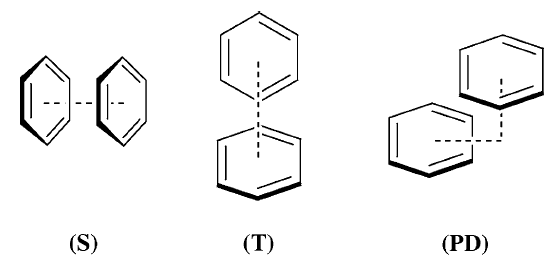
\includegraphics[scale=0.8]{image/Prot} \label{figprot}
   						\caption[Structures du dimère de Benzène]{Structures des dimères de Benzène : (S) Sandwich, (T) En forme de T et (PD) Parallèle Déplacé}
   					\end{figure}
   					
   					L’analyse de ces travaux montre que le débat pour estimer quelle est la conformation la plus stable est loin d’être clos. La majorité des travaux rapportent que ce sont les formes T et PD qui sont les plus stables. Pourtant, intuitivement il ne serait pas illogique de penser que la configuration en sandwich, qui correspond à la superposition maximal des deux monomères, puisse apparaitre comme suffisament stable du fait de la maximisation des interactions dispersives. La configuration parallèle déplacée est, quand à elle, souvent observée dans les expériences réalisées à l’état cristallin de composés purement aromatiques \cite{hunter1991pi,fyfe1997synthetic,rebek1996assembly} ou dans les études cherchant à caractériser les interactions des chaînes latérales aromatiques de protéines \cite{hunter1991pi,burley1985aromatic}.
   					Klemperer et al \cite{janda1975benzene} ont, quand à eux, rapportés que la configuration en T était prédominante à l’état gazeux. D’autres travaux issus de l’analyse des spectres rotationnel d'Arunan et Gutowsky \cite{arunan1993rotational}, en accord avec les études Raman de Henson et al \cite{henson1992raman} rapportent que les structures favorables du dimère du benzène s’approchent de la conformation T sans pour autant la confirmer.\\ 
   					
   					
   					Il existe dans la littérature une très grande variété d’approches concernant l’étude des dimères du benzène.
   					Nous faisons le choix de ne reporter, dans le tableau ci-dessous, que les modélisations conduisant aux résultats, à priori du fait des méthodes employées, les plus précis et qui font référence. Les travaux de Park et Lee \cite{park2006accurate}, de Tsuzuki et al \cite{tsuzuki2002origin} et de Sinnokrot et al \cite{hobza1996potential} ont tous été obtenus a partir de calculs CCSD(T) avec extrapolation CBS de base (en anglais Complete Basis Set extrapolation).
   					Cette méthodologie est une technique de calcul empirique basée sur un minimum de trois calculs séparés avec des bases de plus en plus complètes telles que les bases de type cc-pVXZ (X=T, Q, 5 …). 
   					Cette technique est une estimation approchée d’un résultat obtenu en utilisant une base infini. Elle permet d’atteindre la limite
   					de précision de la méthode de calcul la plus performante.
   					Nous avons reportés dans le tableau les résultats que nous avons obtenus sur la forme PD qui est celle qui à priori nous intéresse en priorité puisque c’est celle qui a été caractérisée expérimentalement à l’état solide (comme le seront les structures que nous aurons à modéliser dans notre travail issus des données IR obtenues en photo acoustiques). On peut remarquer, en accord avec toutes les données actuellement disponibles sur les approches SAPT, que notre valeur d’énergie d’interaction calculée en SAPT(PBE0)/aug-cc-pVTZ est totalement conforme à la valeur attendue. Sans surprise, l’approche SAPT
   					permet donc de reproduire avec une excellente vélocité les énergies d’interaction de systèmes en interaction pi-pi et d’atteindre la précision nécessaire pour reproduire des données aussi faibles que 1 à 2 kcal/mol. 
   					
   					
   					
   					\begin{table}[H]
   						\caption{Energie d'interaction du dimère de Benzène avec CCSD(T) en kcal/mol et DFT-SAPT (PBE0)}
   						\begin{center}
   							\begin{tabular}{l c c c c}
   								\toprule
   								& & T& & PD\\
   								\midrule
   								Park et Lee$^{1}$ & & -2,67& &-3,03\\
   								Tsuzuki et al$^{2}$ & & -2,46& & -2,48\\
   								Sinnokrot et al$^{3}$ & & -2,74& & -2,78\\
   								Hobza et al$^{4}$ & & -2,17& & -2,01\\
   								DFT-SAPT (PBE0) & & & & -2.35\\
   								\bottomrule
   							\end{tabular}
   						\end{center}
   						\centering
   						\footnotemark[1]{ref \cite{park2006accurate}},
   						\footnotemark[2]{ref \cite{tsuzuki2002origin}},
   						\footnotemark[3]{ref \cite{sinnokrot2002estimates}},
   						\footnotemark[4]{ref \cite{hobza1996potential}}
   						
   						[1] CCSD(T)/CBS
   						[2] CCSD(T)/CBS 
   						[3] CCSD(T)/CBS
   						[4] CCSD(T)/aug-cc-pVDZ
   						[5] SAPT(PBE0)/aug-cc-pVTZ
   						
   						
   						\label{benzene}
   					\end{table}
   					



